\section{Case Study}
\label{sec:case-study}

We consider a multi-hop network which has a chain of OpenWSN nodes (see Figure~\ref{fig:multihop}), where each node has a different {\em NodeId} (assigned as an integer), increasing from left to right. 
\begin{figure*}[t]
\centering
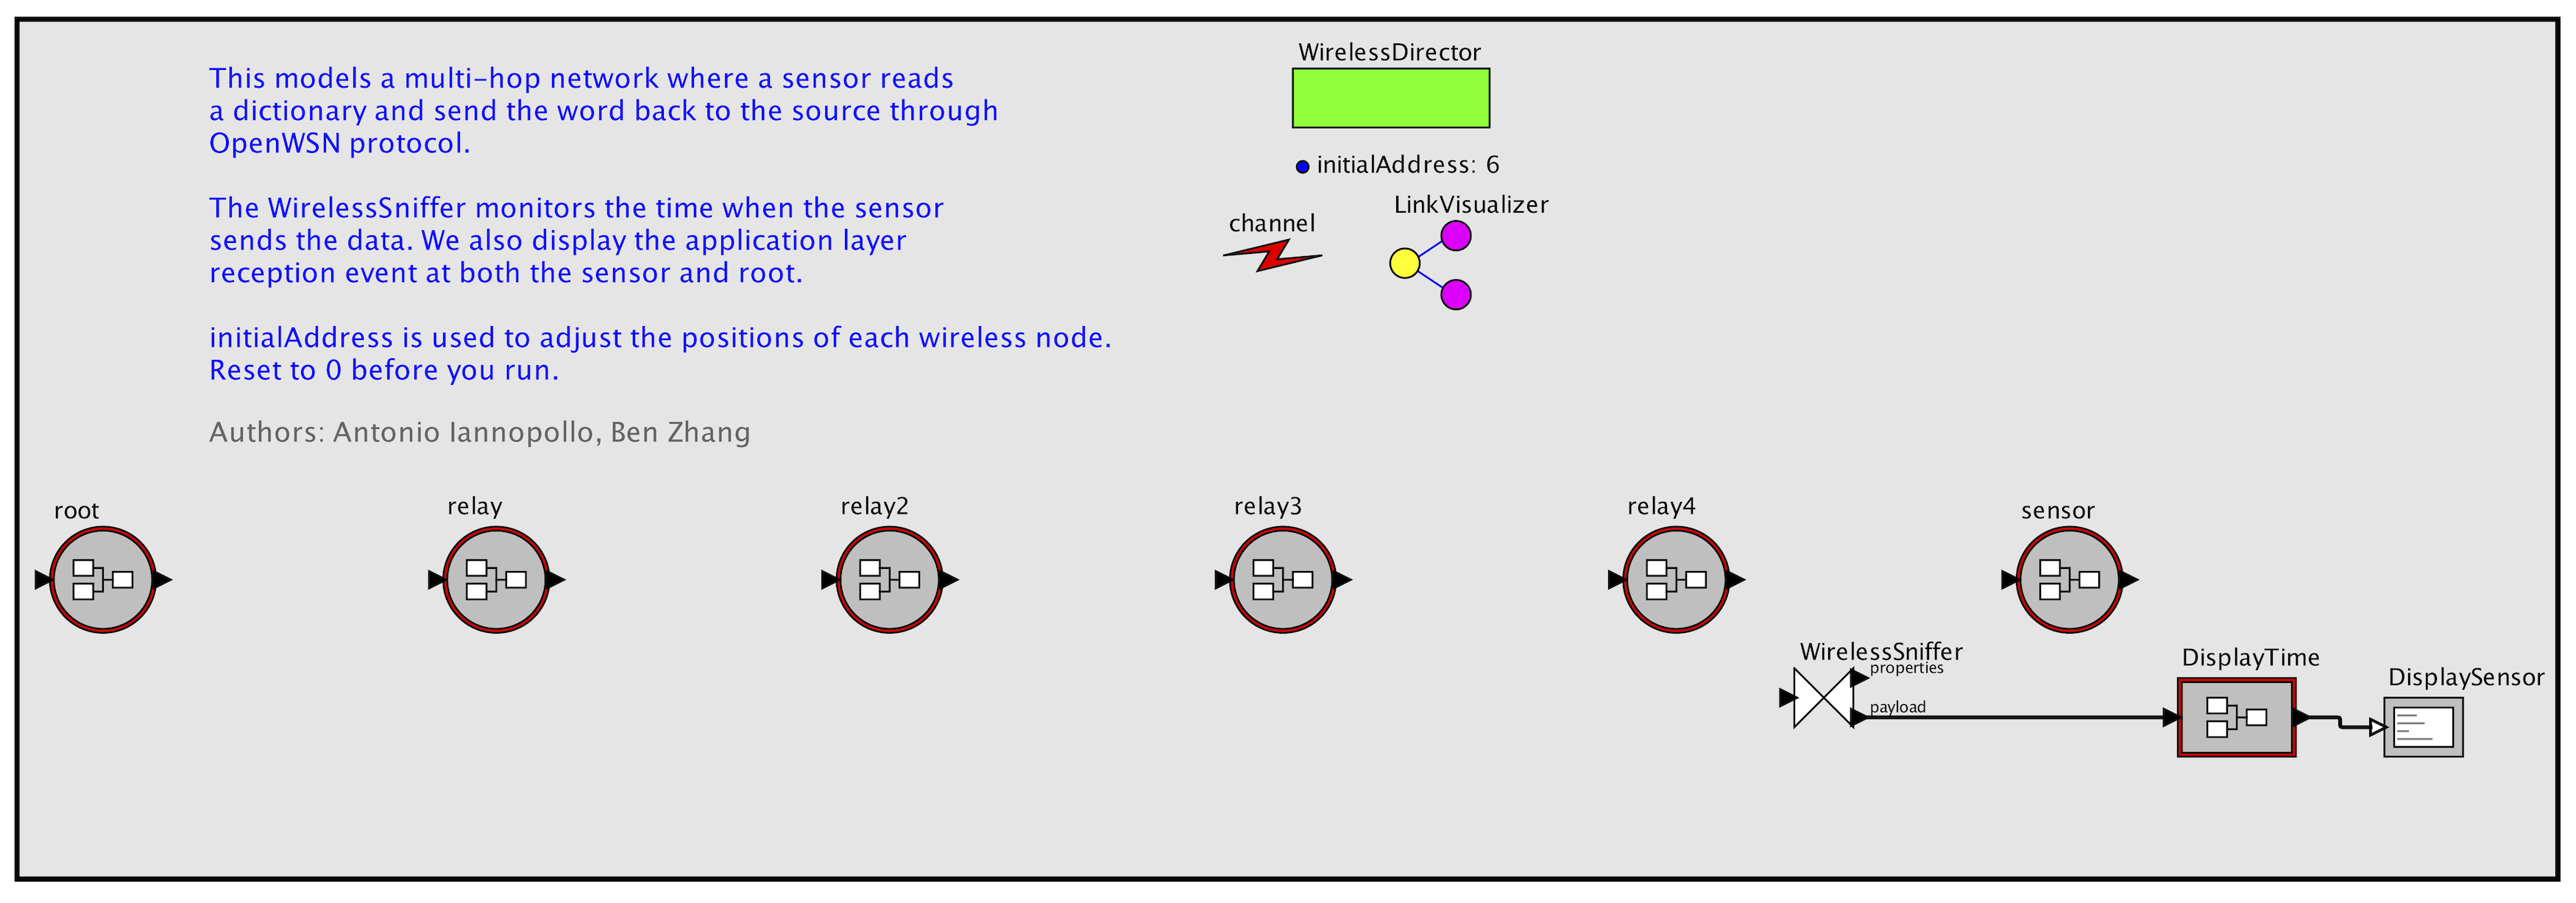
\includegraphics[width=0.8\textwidth]{figures/PaperDemoPtolemy}
\caption{\small A multi-hop OpenWSN network.}
\label{fig:multihop}
\end{figure*}
Node schedules are constructed following the schema:

\begin{tabular}{ l | c | c | c | c | c }
  \hline                       
  NodeId & \multicolumn{5}{c}{Schedules} \\
  \hline
  $3i+0$ & \texttt{ADV} & \texttt{TX} & \texttt{RX} & \texttt{OFF} & $k \times \texttt{OFF}$ \\
  $3i+1$ & \texttt{ADV} & \texttt{RX} & \texttt{OFF} & \texttt{TX} & $k \times \texttt{OFF}$ \\
  $3i+2$ & \texttt{ADV} & \texttt{OFF} & \texttt{TX} & \texttt{RX} & $k \times \texttt{OFF}$ \\
  \hline  
\end{tabular}
where $i \in \mathbb{N}$ and $k$ is specified to control the duty cycle of each node (higher $k$ indicates more \texttt{OFF} slots in the schedule period and thus a lower duty cycle). Intuitively, when $k$ is small, nodes can receive \texttt{ADV} packet in a relatively timely fashion. This helps especially in case of lost synchronization. However, in case of high duty cycle schedules, the price a node needs to pay is to spend more time in \texttt{TX} and \texttt{RX} states, which potentially increases the power consumption. On the other hand, if $k$ is large, nodes that have lost synchronization will have to wait longer, leading to an increased energy consumption caused by turning the radio on and listening for long periods. Schedule duty cycle tuning is a critical activity in order achieve performance while minimizing energy consumption. In this work, we leave a formal study as future work, and only focus on cases when $k = 0, 144, 306$. These values correspond to $\sim0.06$, $\sim2.5$ and $\sim5$ seconds schedule periods. 

\begin{figure}[t]
\centering
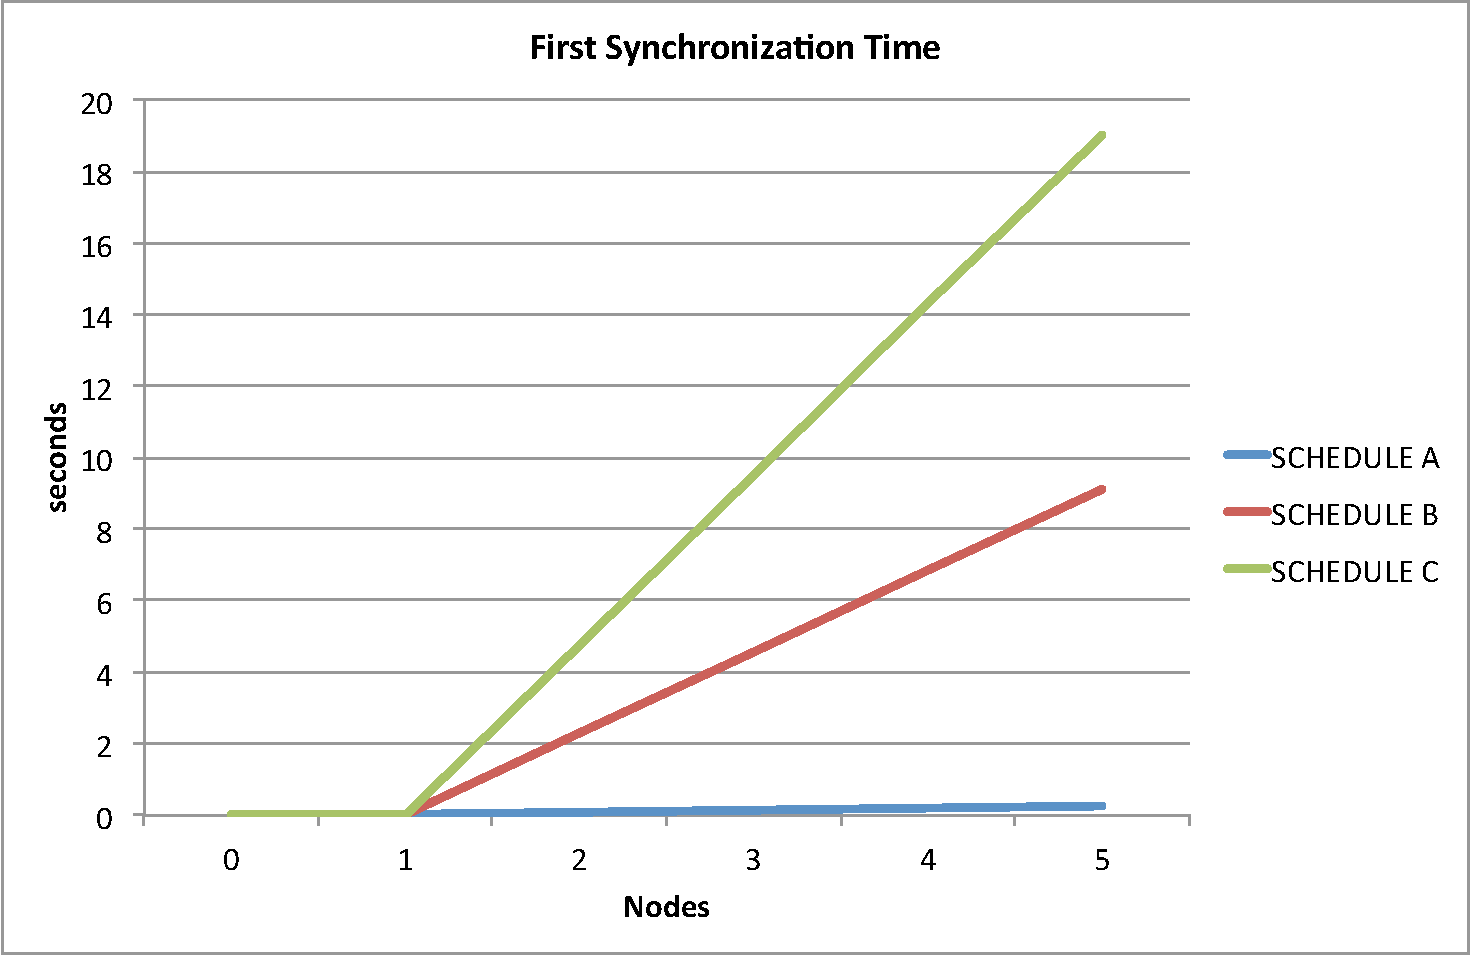
\includegraphics[width=0.9\columnwidth]{figures/synch_time_sched_big}
\caption{\small For each node, the time it first gets synchronized (the time it joins the network).}
\label{fig:time_sync}
\end{figure}

\begin{figure}[t]
\centering
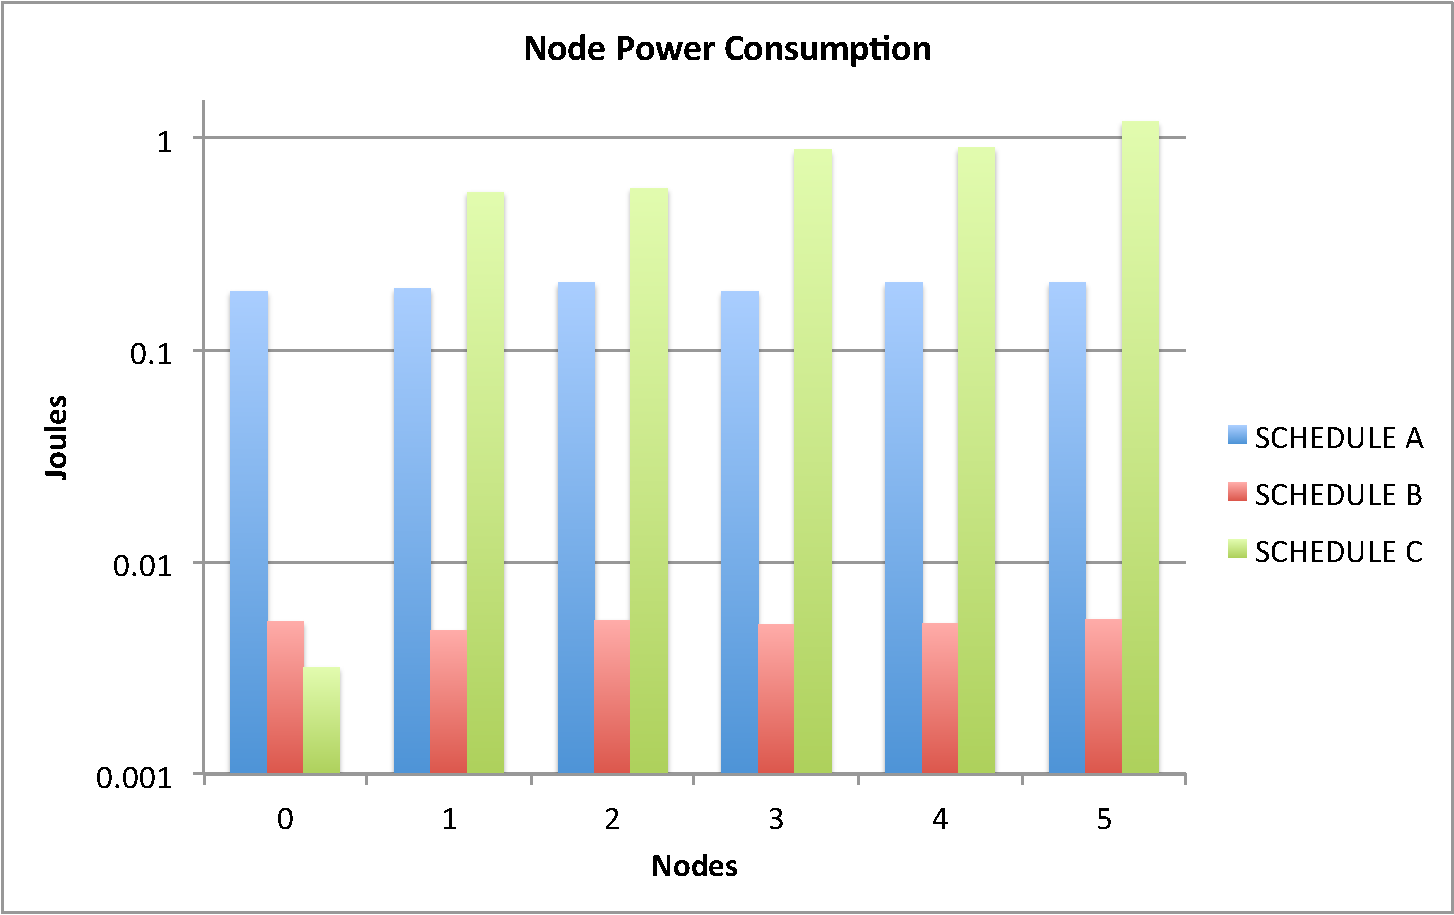
\includegraphics[width=0.9\columnwidth]{figures/power_cons_big}
\caption{\small For each node, the measured power consumption after then network is on for 20 seconds.}
\label{fig:power_evaluation}
\end{figure}

We present the results of a network that has 6 chained nodes under the three different schedules in Figure~\ref{fig:time_sync} and Figure~\ref{fig:power_evaluation}. Here we use two metrics to evaluate each schedule. The first metric is the time of first synchronization for each node in the network. This metric gives us an idea of how \emph{reactive} the network is. The second is the power consumption of each node in the network. This last metric helps to evaluate, among other factors, the overall autonomy of battery-powered network devices, which correlates to the network {\em durability}.
In our experiments we simulated a time window of 20 seconds. We use the Ptolemy \emph{Wireless Director}, a modified version of the \emph{Discrete Event Director} with some additional parameters typical of wireless scenarios.The simulated channel is an ideal one, where the packet loss probability is 0 and signals are propagated with infinite speed.

Looking at Figure~\ref{fig:time_sync}, we see that the first synchronization time is proportional to the relative distance of each node from the root (as the reader intuition suggests). In case of higher duty cycle, when $k$ is smaller (such as with Schedule A), each node waits for a shorter time to reach synchronization. 

On the other hand, considering the network power consumption, we have found that if the duty cycle is high ($k$ is small), then most nodes are busy in \texttt{TX} and \texttt{RX} states, leading to similar energy consumption values. When the duty cycle is low, then nodes that are farther from the root tend to stay longer in the \texttt{synchronization} state (because of the less frequent \texttt{ADV} packets), resulting in longer times with the radio in listening mode. Interestingly, schedules with a moderate duty cycle (see Schedule B), where transmissions are less frequent but not in a way to cause node de-synchronization, lead to an overall smaller amount of energy consumption.

\subsection{Model Scalability}
\label{sec:scalability}

To test model scalability, we performed several additional experiments considering different conditions.
We used two model configurations. In the first case , the model computed the power consumption estimation for each node during execution. In the second one, the power consumption estimation feature was disabled.
For each configuration, we considered the same network characteristics and the same topology \emph{style} as in section~\ref{sec:case-study}. The only difference was the number of nodes involved in the simulations. In particular, we had chains of 6, 20 and 50 nodes.
For all experiments, we simulated 10 seconds of execution.
Experiments have been run on a 8 cores, 3.70GHz Intel(R) Xeon(R)-based machine with 32GB of RAM.

\begin{figure}[t]
\centering
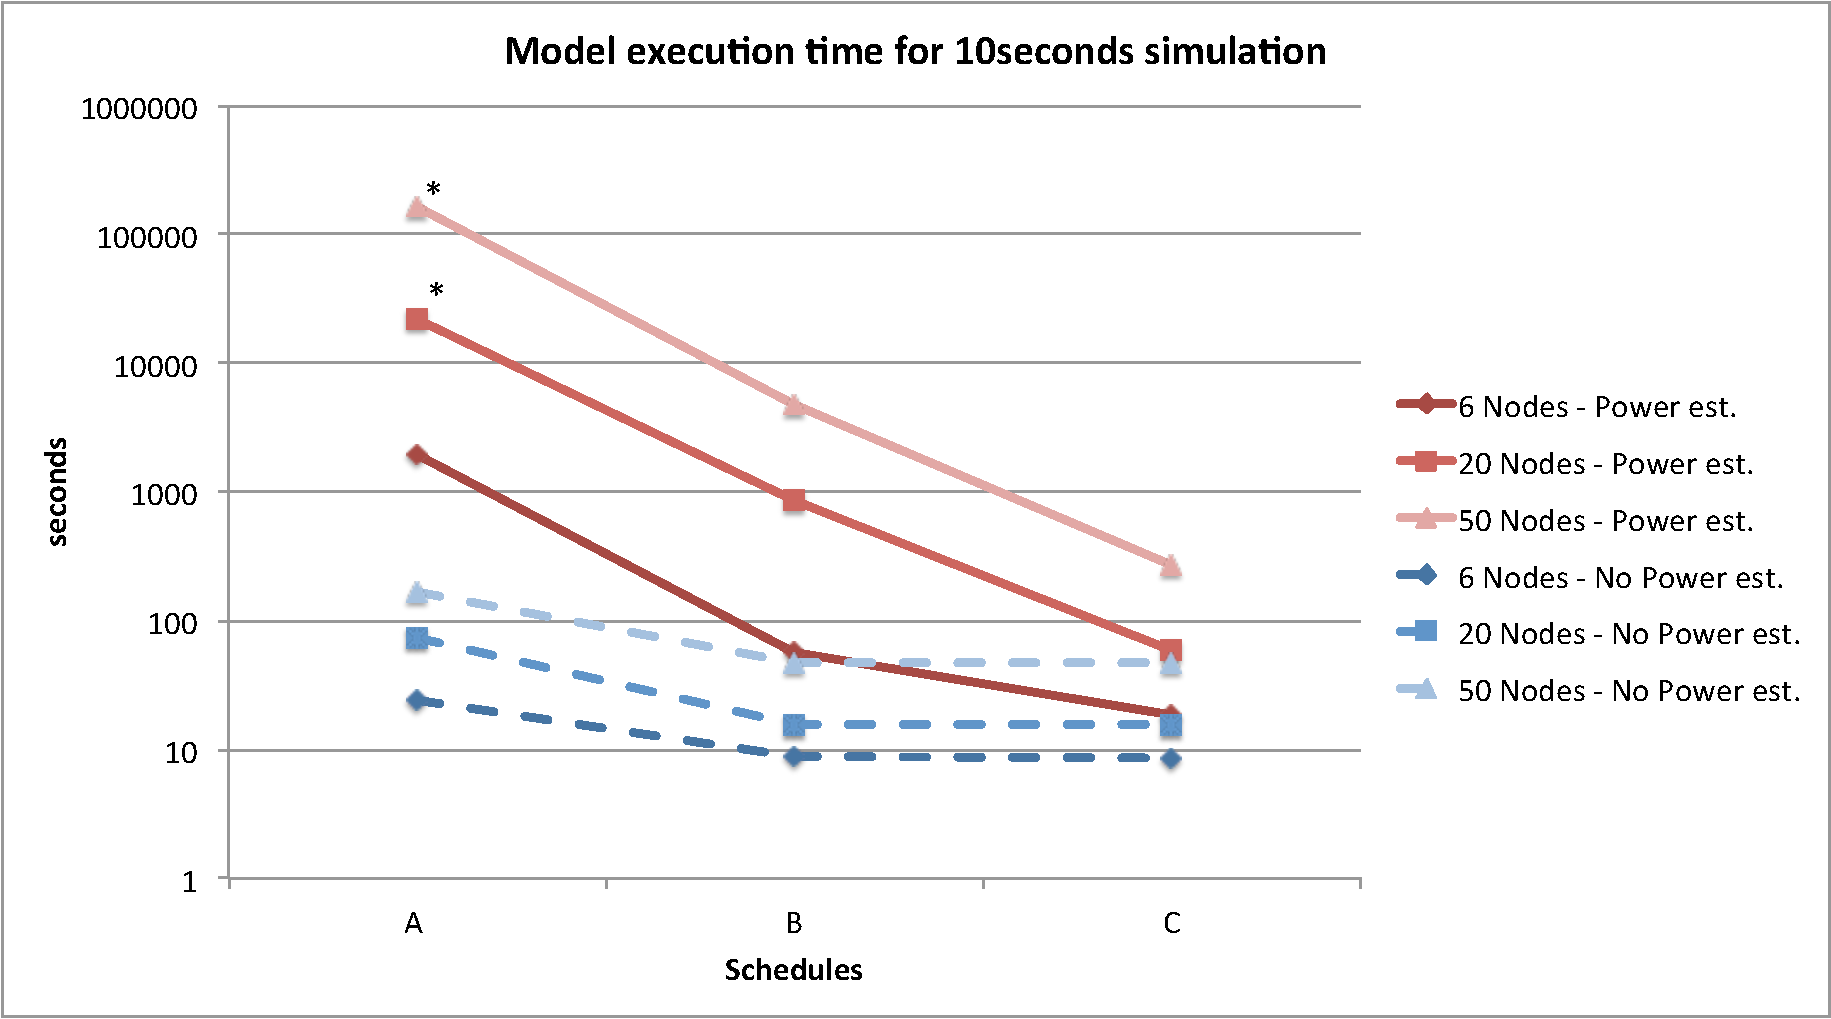
\includegraphics[width=0.9\columnwidth]{figures/runtime}
\caption{\small Model execution time for a simulation of 10 seconds with different number of nodes and different model configurations (with and without power estimation). Points marked with the \emph{*} symbol are estimated from incomplete data, after a 60 minutes execution timeout.}
\label{fig:runtime}
\end{figure}

Figure~\ref{fig:runtime} shows results relative to the execution of the models.
Analyzing results, the first observation is the relevant impact of the power estimation feature of the model on the total execution time.
On the other hand, we can see how also the choice of the schedule has an important influence on the execution time.
Overall, considering schedules with low duty cycle (common in practical applications), we observed a reasonable execution time in computing a precise power consumption estimation even for big networks.
Interestingly, excluding the power consumption estimation feature from the model, we obtain good execution times also in case of very high duty cycle schedules and high number of nodes in the network.
 



%%% Local Variables: 
%%% mode: latex
%%% TeX-master: "ee219d"
%%% End: 
